%! TEX program = LuaTeX

\documentclass[nobackground,dvipsnames,table]{beamer}
\usepackage{sio}

\mode<presentation>
{\usetheme{Hannover}
    \usecolortheme{sio}
    \setbeamercovered{transparent}
    \useinnertheme[shadow=false]{rounded}
    \usebackgroundtemplate{}
    \setbeamercolor*{frametitle}{parent=palette primary}
    \setbeamerfont{block title}{size={}}
    \setbeamertemplate{navigation symbols}{}
}

\title{Authentication and Identity}
\subtitle{CS 152: Trust and Safety Engineering}

\author[A. Stamos]{Alex Stamos}
\institute[SIO]{\large Stanford Internet Observatory}
\date[2022]{\today}
\subject{CS 152 - Trust and Safety Engineering}
\titlegraphic{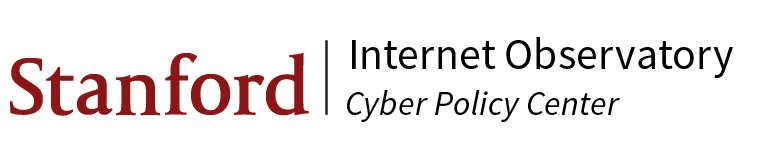
\includegraphics[width=5cm]{img/internet-observatory}}

% Change the level of bulleting on the ToC page
\setcounter{tocdepth}{2}

\graphicspath{{/img/lesson03}}

\begin{document}

\coverpage

\begin{frame}
    \titlepage
\end{frame}

\begin{frame}{Twitter Hack}
    
\end{frame}

\begin{frame}{What Will You Learn Today?}
    \begin{itemize}
        \item Digital identity relationships
        \item Basic and Advanced Authentication Flows
        \item Threats to Authentication
        \item Defense Against the Dark Arts
        \item Emerging Threats
    \end{itemize}
\end{frame}

\begin{frame}{Digital Identity Mappings}
    %TODO Diagram
\end{frame}

\begin{frame}{Account <-> Real Human}
    \begin{itemize}
        \item Impersonating accounts
        \item Romance scams
        \item Advance fee fraud
        \item Physical good fraud
    \end{itemize}
    %TODO photos
\end{frame}

\begin{frame}{User <-> Account}
    %TODO pictures
    \begin{itemize}
        \item Stealing passwords
        \item Cracked breached password databases
        \item Credential stuffing
        \item Malware (Trojans)
    \end{itemize}
\end{frame}

\begin{frame}{Organization <-> Infrastructure }
    \begin{itemize}
        \item Phishing 
        \item Meddler-In-The Middle (MITM) attacks
        \item Typosquatting
        \item Mismatched domains
        \item Internationalized Domain Name (IDN) Homograph attack
        \item Email security
    \end{itemize}
    %TODO image
\end{frame}

\begin{frame}{Black Markets Allow For Specialization of Effort}
    There are:
        \begin{itemize}
            \item Markets for stolen data
            \item Easy-to-use malware, like keyloggers 
            \item Phishing kits
            \item Hackers for hire
            \item Botnets 
        \end{itemize}
%TODO images
\end{frame}

\begin{frame}{Why Should I Care?}
    There are multiple levels of identity online and strong authentication is essential for them all. \\
    Protecting users while maintaining availability requires a complex web of systems covering Prevention, Detection, and Mitigation.
\end{frame}


%TODO2 Should I put in slides that are skipped in presentation mode?

%TODO authn vs authz slide

\begin{frame}{How Does Authentication Work?}
    
\end{frame}

\begin{frame}{How Does Authentication Work?}
    
\end{frame}

\begin{frame}{How Does Authentication Work?}
    
\end{frame}

\begin{frame}{How Does Authentication Work?}
    
\end{frame}

\begin{frame}{Multi-factor}
    
\end{frame}

\begin{frame}{} %Something you have, something you know, something you are
    
\end{frame}

\begin{frame}{}
    
\end{frame}

\begin{frame}{Adoption of Security Measures}
    
\end{frame}

\begin{frame}{Threats}
    \begin{itemize}
        \item Credential breach
        \item Malware
        \item Phishing
        \item Active MITM
    \end{itemize}
\end{frame}

\begin{frame}{Quota Inversion}
    Initial account hijacking was just phishing \\
    Ten failed logins per password vs ten failed logins per account\\
    Mass market attacker who just wants to send out links to viagra just needs to get into any account - they don’t care which one\\

    Different world - weaponized targeted account for a specific adversary
\end{frame}

\begin{frame}{Quota Inversion}
    
\end{frame}

\begin{frame}{Quota Inversion}
    
\end{frame}

\begin{frame}{Credential Breach}
    
\end{frame}

\begin{frame}{Likelihood of Compromise}
    
\end{frame}

\begin{frame}{Likelihood of Compromise}
    
\end{frame}

\begin{frame}{}
    
\end{frame}

\begin{frame}{}
    
\end{frame}

\begin{frame}{}
    
\end{frame}

\begin{frame}{}
    
\end{frame}

\begin{frame}{}
    
\end{frame}

\begin{frame}{}
    
\end{frame}

\begin{frame}{}
    
\end{frame}

\begin{frame}{}
    
\end{frame}

\begin{frame}{}
    
\end{frame}

\begin{frame}{}
    
\end{frame}

\begin{frame}{}
    
\end{frame}

\begin{frame}{}
    
\end{frame}

\begin{frame}{}
    
\end{frame}

\begin{frame}{}
    
\end{frame}

\begin{frame}{Mitigation}
    Risk-based authentication challenges\\
    Implicit signals\\
    Strong authentication\\
    Federation
\end{frame}

\begin{frame}{Sign-in Risk Detection}
    \begin{columns}
        \column{0.6\textwidth}
            \begin{itemize}
                \item Unusual location, device, time, network 
                \item Phishing history
                \item Similarity to known account hijacking patterns (number of login attempts, sensitivity of info accessed, etc.)
                \item \textit{The higher the estimated probability that the login attempt is fraudulent, the more multi-factor authentication steps should be required of the user.}
            \end{itemize}
            %TODO graphics
        \column{0.4\textwidth}
            %TODO image
    \end{columns}
\end{frame}

\begin{frame}{Detecting Hijacker In-session}
    
\end{frame}

\begin{frame}{Detecting Hijacker In-session}
    
\end{frame}

\begin{frame}{Detecting Hijacker In-session}
    
\end{frame}

\begin{frame}{Detecting Hijacker In-session}
    
\end{frame}

\begin{frame}{Authentication Beyond Passwords}
    
\end{frame}

\begin{frame}{}
    
\end{frame}

\begin{frame}{}
    
\end{frame}

\begin{frame}{Identity Federation}
    
\end{frame}

\begin{frame}{Identity Federation}
    
\end{frame}

\begin{frame}{}
    
\end{frame}

\begin{frame}{Exotic Attacks}
    \begin{itemize}
        \item OAuth Phishing
        \item Token Theft
    \end{itemize}
\end{frame}

\begin{frame}{OAuth}
    
\end{frame}

\begin{frame}{}
    
\end{frame}

\begin{frame}{}
    
\end{frame}

\begin{frame}{Stealing Access Tokens}
    
\end{frame}

\begin{frame}{}
    
\end{frame}

\begin{frame}{Risk and Incident Sharing and Coordination}
    
\end{frame}

\begin{frame}{Where Is This Going?}
    After taking over an account, what do the attackers do?\\
    Over the next few weeks, we’ll cover the spectrum from simple, commercial monetization, to more nuanced forms of reputation hijacking, to data theft and weaponization
\end{frame}

\begin{frame}{Review}
    
\end{frame}

\begin{frame}{}
    
\end{frame}

\begin{frame}{What Will We Learn Today?}
    
\end{frame}

\begin{frame}{Credential Breach}
    
\end{frame}


\backpage

\end{document}
